\section{Testy statystyczne: FULLMATRIX dla 2-opt i rozszerzonego sąsiada}
  \subsection{Cel:}
  Typ danych FULLMATRIX zmienia zasady gry, gdyż w tego typu przykładach nierówność trójkatą nie musi być zachowana. Celem tego etapu jest sprawdzenie reakcji algorytmów na nowy typ danych
  \subsection{Założenia:}
  Do tego badania użyto automatycznie wygenerowanych grafów typu \textbf{FULL MATRIX}. Rozmiary grafów (oznaczane literą n) należą do zbioru $n \in \{10,15,20,...,100\}$. Dla algorytmu 2-opt element startowy został automatycznie wygenerowany.
  \subsection{Wyniki: }
  \begin{table}[H]
    \begin{tabular}{|c | c | c |} 
     \hline
     n & 2-OPT & RozszerzonySąsiad \\ [0.5ex] 
     \hline\hline
    10 & 266 & 193 \\
    15 & 300 & 252 \\
    20 & 400 & 265 \\
    25 & 498 & 271 \\
    30 & 541 & 239 \\
    35 & 492 & 272 \\
    40 & 512 & 261 \\
    45 & 534 & 306 \\
    50 & 600 & 310 \\
    55 & 580 & 370 \\
    60 & 534 & 252 \\
    65 & 780 & 323 \\
    70 & 678 & 316 \\
    75 & 800 & 286 \\
    80 & 995 & 357 \\
    85 & 1141 & 432 \\ 
    90 & 1110 & 352 \\
    95 & 1251 & 384 \\ 
    100 & 1399 & 396 \\

     \hline
    \end{tabular}
    \caption{Funkcje celu dla wybranych algorytmów.}
    \end{table}
  \subsection{Wykresy: }
  \begin{figure}[H]
      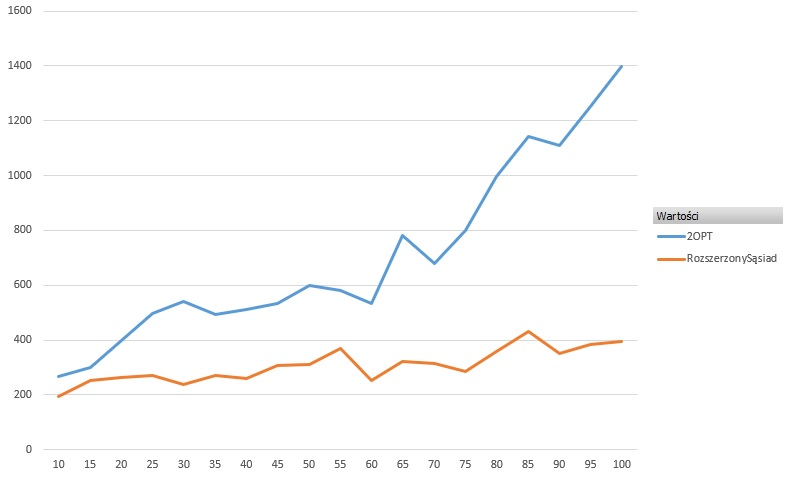
\includegraphics[scale=0.75]{fullmatrixOPT}
      \centering
      \caption{Funkcja celu dla 2-opt dla różnych startowych permutacji}
    \end{figure}


  \subsection{Test statystyczny Wilcoxona: }
    \textbf{Hipoteza zerowa: $OPT =< ENN$}, gdzie OPT oznacza algorytm 2-opt, a ENN- rozszerzony algorytm najbliższego sąsiada. \\
    \textbf{Hipoteza alternatywna: $OPT > ENN$ }
    \begin{table}
    \begin{tabular}{|c | c | c | c | c | c |} 
     \hline
     Pair & OPT & ENN & Abs.Diff & Rank & Sign \\ [0.5ex] 
     \hline\hline
      2 & 300 & 252 & 48 & 1 & +1 \\
      1 & 266 & 193 & 73 & 2 & +1 \\
      3 &  400 & 265 & 135 & 3 & +1 \\
      10 & 580 & 370 & 210 & 4 & +1 \\
      6 & 492 & 272 & 220 & 5 & +1 \\
      4 & 498 & 271 & 227 & 6 & +1 \\
      8 & 534 & 306 & 228 & 7 & +1 \\
      7 & 512 & 261 & 251 & 8 & +1 \\
      11 & 534 & 252 & 282 & 9 & +1 \\
      9 & 600 & 310 & 290 & 10 & +1 \\
      5 & 541 & 239 & 302 & 11 & +1 \\
      13 & 678 & 316 & 362 & 12 & +1 \\
      12 & 780 & 323 & 457 & 13 & +1 \\
      14 & 800 & 286 & 514 & 14 & +1 \\
      15 & 995 & 357 & 638 & 15 & +1 \\
      16 & 1141 & 432 & 709 & 16 & +1 \\
      17& 1110 & 352 & 758 & 17 & +1 \\
      18& 1251 &384  & 867 & 18 & +1 \\
      19& 1399 & 396 & 1003 & 19 & +1 \\
     \hline
    \end{tabular}
    \caption{Tabela rang dla testu Wilcoxona}
    \end{table}

    $W_{-} = 0$.\\
    $W_{+} = 190$. \\
  \subsection{Wnioski: }
    Wartość krytyczna $\alpha = 0.05$. Dla tego typu statystyk $T_{crit}=53$ (dana z tabeli dla hipotez "o jednym ogonie"). Hipoteza zerowa jest odrzucona, gdy $ T \leq 53 $. U nas $T=0$, jako minimum z $W_{-} i W_{+}$, więc hipoteza zerowa zostaje odrzucona.